\chapter{Calorimetry and dual-readout}
Calorimetry is an important detection principle in particle physics.
Originally developed with astrophysical purpose for cosmic-ray studies, this method refers to the detection of particles and the measurement of their properties, using blocks of instrumented material.
It was developed and perfected for accelerator-based particle physics experimentation primarily in order to measure the energy of particles. 
In these blocks, particles are fully absorbed and their energy transformed into a measurable quantity.\\
The incident particle interact with the detector (through electromagnetic or strong processes) producing a shower of secondary particles with progressively degraded energy.
The energy deposited by the charged particles of the shower in the active material of the calorimeter, which can be detected in the form of charge or light, is used to measure the energy of the incident particle.
Typical processes suitable to detect this energy are: ionization of the medium, scintillation light and the Cherenkov light produced by relativistic particles.\\

Calorimeters can be divided into two categories depending on the type of shower they are optimized to detect: electromagnetic calorimeters, used mainly to measure electrons and photons through their electromagnetic interactions (e.g.
bremsstrahlung, pair production), and hadronic calorimeters, used to measure mainly hadrons through their strong and electromagnetic interactions.\\
Another classification can be made according to their construction technique defining sampling calorimeters and homogeneous calorimeters.\\
Homogeneous calorimeters are built of one type of material that performs both the main tasks: degrade the energy of the incident particles and provide the detectable signal.\\
Sampling calorimeters, instead, consist of alternating layers of an absorber, a dense material used to perform energy degradation, and an active medium that generate the signal.\\

%Calorimeters are attractive in high-energy particle physic field for various reasons:
%\begin{itemize}
%		\item In most cases the calorimeter energy resolution improves with energy as $1/\sqrt{E}$, where $E$ is the energy of the incident particle. Therefore calorimeters are very well suited to high-energy physics experiments.
%		\item Calorimeters are sensitive to all types of particles, charged and neutral (e.g., neutrons). Also neutrinos and their energy can be indirectly detected can even provide indirect detection of neutrinos and their energy through the measurement of the event missing energy.
%		\item They are versatile detectors. They can be used to determine the shower position and direction, to perform particle identification, to measure the arrival time of the particle, or even to provide fast signals useful in trigger purpose.
%		\item They are space and therefore cost effective. Because the shower length increases only logarithmically with energy, the detector thickness needs to increase only logarithmically with the energy of the particles.
%\end{itemize}

This chapter describes the physics behind both the electromagnetic and hadronic shower developments, provides a basic description of the energy response of these detectors and introduces the particular technique of the dual-readout, a modern concept of calorimeter that has the quality of overcome the non-compensating problem measuring both electromagnetic and hadronic showers through two different type of signals simultaneously (Cherenkov and scintillation light).\\

A more comprehensive descriptions of the topic can be found in the references \cite{Wigmans_book, Wigmans_art_of_cal, Gianotti_article}.

\section{Physics of shower development}
A particle interact and lose part or whole of its energy traversing matter. During this process the medium get excited and heated up. From this feature the term calorimetry, literally meaning ``heat measurement", was introduced.\\
The groundwork for the calorimetry is the interaction processes between particle and matter. They are the manifestation of the electromagnetic, the strong and, more rarely, the weak forces and they strongly depend on the energy and the nature of the incident particle, in addition to medium features.\\
The term particle shower refers to the production of a group of particles generated by the interaction of a primary particle with the matter. The processes and the consequent shower effects are the keys to deeply understand this topic.\\

\subsection{Electromagnetic showers} \label{subsec:em_shower}
Despite the complex mechanisms of particle-matter interaction, electromagnetic showers are produced via a small number of well understood QED processes. Charged particles (electrons and positrons) lose energy by ionization and by radiation, instead neutral ones (photons) are characterized by photoelectric effect, Compton scattering and pair production.\\

The first type of particle ionize the medium, in its path through it, under the condition of having an energy at least sufficient to release the atomic electrons from the Coulomb fields generated by the atomic nuclei (few of $eV$).
The amount of energy released (in unit of path) by these particle is predictable through the semi-empirical Bethe-Block formula restricted to electrons (and positrons) \cite{Leo}:
\begin{equation}
    -\frac{dE}{dx} = 2\pi N_a r_e^2 m_e c^2 \rho \frac{Z}{A}\frac{1}{\beta^2}\left[ \ln{\frac{\tau^2(\tau + 2)}{2(I/m_ec^2)^2}} -F(\tau) -\delta -2\frac{C}{Z}\right].
\end{equation}
The stopping power (i.e. the quantity described by the formula) decreases as the particle energy increases ($\propto \beta^2$). Hence the ionization process is the greatest source of energy loss for particles with small energy.\\
The other energy loss process known as \textit{bremsstrahlung} is the dominant source of energy loss by electrons and positrons at energies above $100\ MeV$. Relativistic electrons and positrons radiate photons as a result of the interaction between Coulomb and the atomic electric fields. The energy spectrum of these photons falls off as $1/E$ ranging till the primary particle energy, but in general most of the photons carry a small part of it.
The process produces (usually small) changes in electron (or positron) direction. This is called Coulomb or multiple scattering.\\
At a fixed energy the relative importance of ionization and radiation losses depends on the medium and in particular on the electron density of the medium in which the shower develops. This density is in first approximation proportional to the $Z$ of the medium.
The critical energy, i.e. the energy value at which the two processes have equal impact, is roughly inversely proportional to the $Z$ value of the material:
\begin{equation}
    \varepsilon_c = \frac{160\ MeV}{Z + 1.24}.
\end{equation}
An example of energy loss in copper by electron is sketched in figure \ref{fig:Cu_rad_ion}, where the ionization and radiation contribution are separated.\\

\begin{figure}
	\centering
	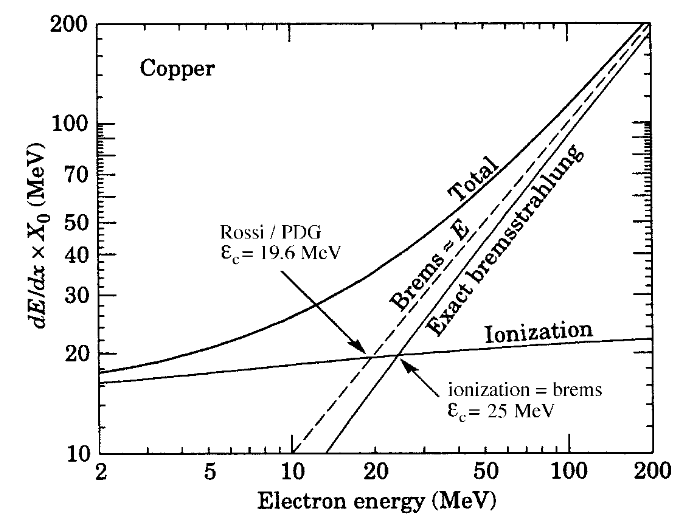
\includegraphics[width=0.8\textwidth]{IMG/Cap2/Cu_rad_ion}
	\caption{Energy losses through ionization and bremsstrahlung by  electrons in copper \cite{PDG_98}}
	\label{fig:Cu_rad_ion}
\end{figure}

The other particles that produce electromagnetic showers are photons. The interaction between photons and matter is mainly affected by three different processes: the photoelectric effect, Compton scattering and electron–positron pair production.\\
The photoelectric effect is the process that most likely occurs at low energies. It is characterized by an atom absorbing the photon and emitting an electron. Eventually the atom, left in an excited state, emits an Auger electrons or X-rays returning to the ground state. The photoelectric cross section strongly depends on the available number of  electrons,  and  thus  on  the $Z$ value  of  the  absorber  material. In particular it scales with $Z^n$, with the power $n$ between 4 and 5. Meanwhile the photoelectric cross section rapidly decrease with greater energies, varying as $E^{-3}$. In this way the process rapidly loses its impact as the energy increases. %Quantitatively, in uranium ($Z=92$) the cross section for photoelectric effect is dominant for energies below $700\ keV$, meanwhile for iron  ($Z=26$) decreases his importance from $100\ keV$.\\

The Compton process is a scattering process where an impinging  photon interact with an atomic electron transferring enough momentum and energy to the struck electron to escape from the atomic Coulomb field. Kinematic variables such as energy transfer and scattering angles can be easily obtained applying the laws of energy and momentum conservation. 
% The dynamic is illustrated in Figure \ref{fig:scatt_kin}. 

%\begin{figure}
%	\centering
%	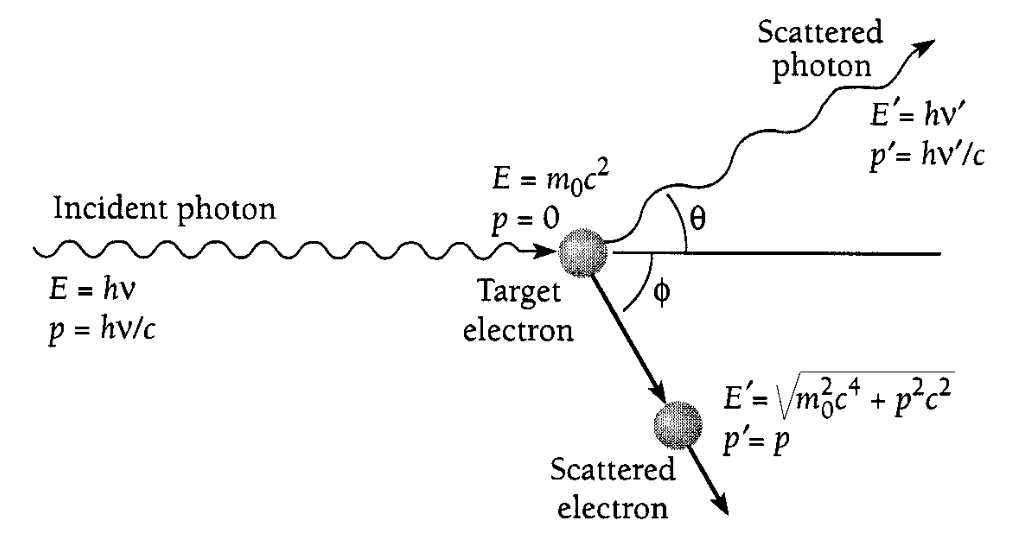
\includegraphics[width=0.8\textwidth]{IMG/Cap2/scatt_kin.png}
%	\caption{Compton scattering process. Image from \cite{Leo}.}
%	\label{fig:scatt_kin}
%\end{figure}

%The photon is absorbed and thus disappears in the photoelectric effect, but it only plays a role at low $\gamma$ energies.
Photons in the $MeV$ energy range are absorbed by photoelectric effect only after a sequence of Compton scattering processes, in which the photon energy is reduced step by step in each collision until it is low enough to permit the photoelectric occurrence. In each step, the amount of loss energy is:
\begin{equation}
    T = E_{\gamma}\frac{\xi(1 - \cos{\theta})}{1 + \xi(1 - \cos{\theta})}
\end{equation}
where $\xi = E_{\gamma}/m_ec^2$.
The cross section linked to the Compton scattering is much less dependent on the $Z$ value than the photoelectric one. It is almost proportional to the number of target electrons in the nuclei. Also in this process the cross section decreases with increasing photon energy, but only with the first power of $E$. Therefore Compton scattering has more impact than photoelectric absorption above a certain threshold energy. %This  threshold varies from $20\ keV$ for carbon ($Z=6$) to $700\ keV$ for uranium ($Z=92$).\\

The pair production process, differently from the previous ones, has a binding threshold under which the effect can not occur. This threshold is the twice of the electron rest mass ($2\times 511\ MeV$). If the photon has a higher energy then it can produce an electron-positron pair that can continue the path in the medium producing bremsstrahlung radiation as well as ionization.
%The electron can be eventually absorbed by an ion, while the positron annihilates with an electron producing two new photons, each with an energy of $511\ keV$.
The cross section for pair production rises with the energy reaching an asymptotic value at energies higher then $1\ GeV$. For this reason, at high energies, pair production is the most likely process to occur. Meanwhile the dependence from the medium goes, in first approximation, as $Z^2$.\\

Comparing the cross section of the three processes and its dependence with respect to the photon energy it is clear that the photoelectric effect dominates at lower energies, meanwhile at the intermediate values the Compton scattering gives the greatest contribute, at the end at higher energies almost every photon is converted in charged particles through pair production. An example of these contributions is shown in figure \ref{fig:ph_cross_E}.\\
Knowing the dependence of the cross sections with respect to the $Z$ of the material, ranges of energies where each process dominates can be found and parametrized with the $Z$ value. A representation is sketched in figure \ref{fig:ph_cross_Z}.

%\begin{figure}
%	\centering
%	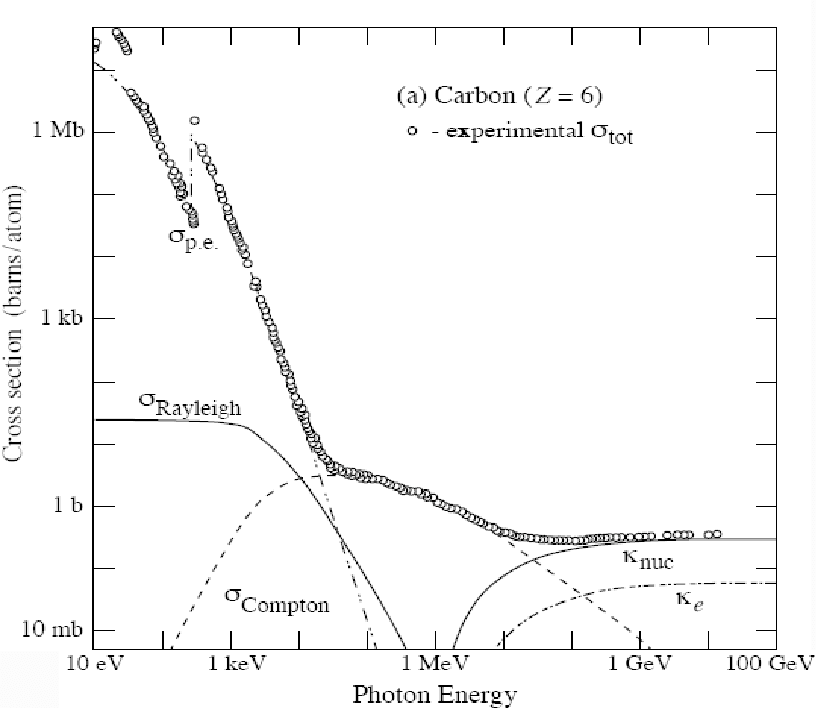
\includegraphics[width=0.7\textwidth]{IMG/Cap2/ph_cross_E.png}
%	\caption{Compton scattering process. Image from \cite{Leo}.}
%	\label{fig:ph_cross_E}
%\end{figure}
%\begin{figure}
%	\centering
%	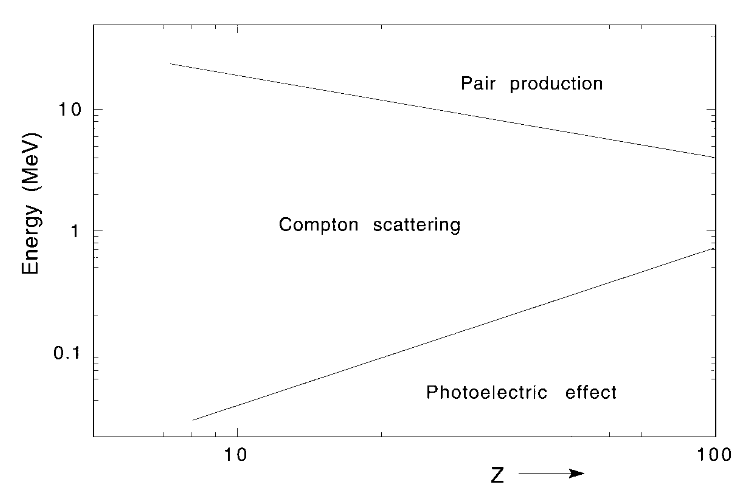
\includegraphics[width=0.7\textwidth]{IMG/Cap2/ph_cross_Z.png}
%	\caption{Compton scattering process. Image from \cite{Leo}.}
%	\label{fig:ph_cross_Z}
%\end{figure}

\begin{figure}
	\centering
	\subfloat[][Total cross section of photon in Carbon. Different processes contribution are also separated. \label{fig:ph_cross_E}]{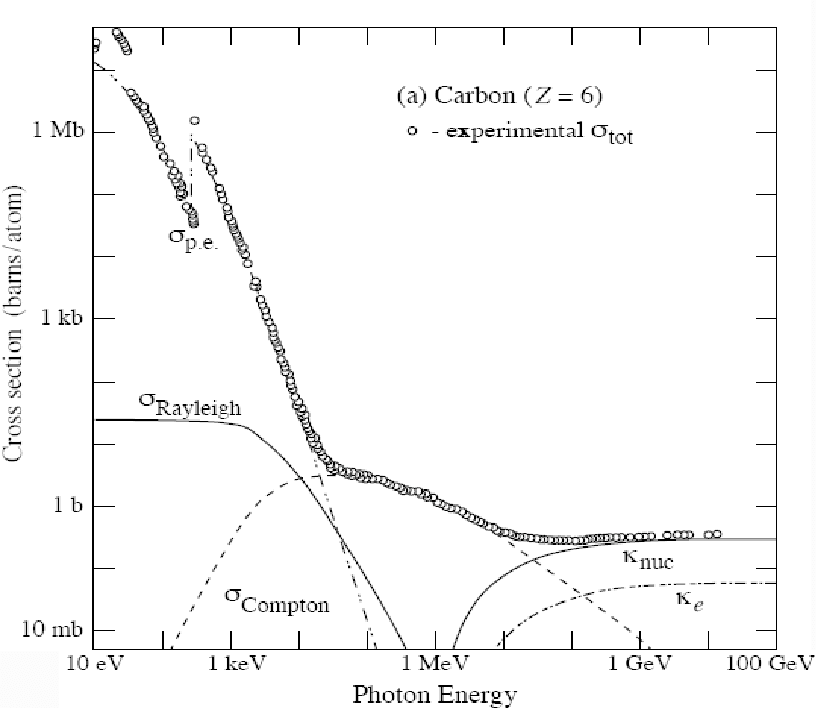
\includegraphics[height=.18\textheight]{IMG/Cap2/ph_cross_E.png}} \quad
	\subfloat[][Energy ranges where different processes dominate with respect to the medium $Z$ value.\label{fig:ph_cross_Z}]{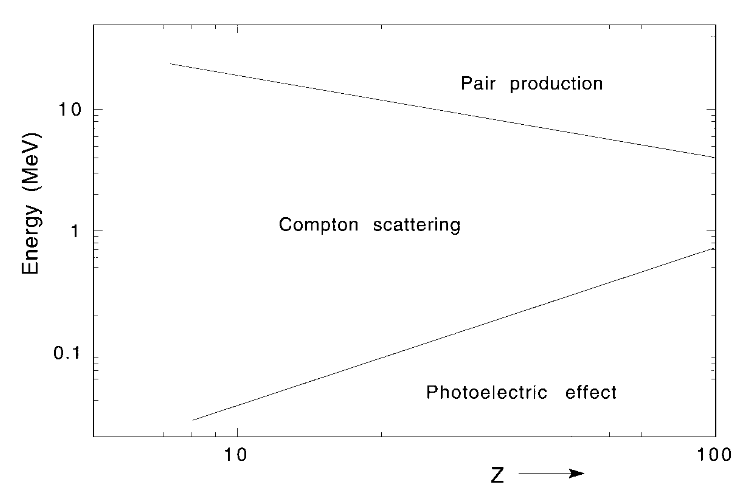
\includegraphics[height=.18\textheight]{IMG/Cap2/ph_cross_Z.png}}
	\caption{Images from \cite{Leo}.}
	%\label{fig:sigma_su_e}
\end{figure}

\subsubsection*{Shower principle}
Minimal showers may also develop at very low energy of primary particle. Starting for example from a photon of tens of $MeV$, it can eventually produce a electron-positron pair in the calorimeter. The  charged  particles lose their energy in the matter through ionization. When the  positron loses all the kinetic energy, it annihilates with an electron producing two $511\ keV\ \gamma$s. These photons are absorbed through the photoelectric effect after a sequence of Compton scattering. During the process, the energy of the primary particle is released to the material by charged particle in ionization processes.\\
At energy values of $1\ GeV$ and higher, electrons, protons and photons initiate actual electromagnetic showers in the materials in which they penetrate. At these energies charged particles lose their energy mostly by brehemstralung, the majority of these photons are very soft, and interact with Compton scattering until their absorption through photoelectric effect. Meanwhile the photons with energy more than $5–10\ MeV$ produce $e^+-e^-$ pairs, which eventually radiate more $\gamma$s. The process continues till the secondary particles energy is higher enough to sustain it. The shower maximum is defined as the point at which the number of shower particles produced in this particle multiplication process reaches a maximum. The depth inside the absorber associated to the shower maximum increases logarithmically with the energy of the primary particle (see figure \ref{fig:shower_max}). The longitudinal shower development is described by the radiation length ($X_0$), it is defined as the distance at which the electron (or positron) loses on average $63\%\ (1-e^{-1})$ of its energy by radiation. Expressing the shower containment in term of $X_0$ helps to mitigate the material-dependence effects.

\begin{figure}
	\centering
	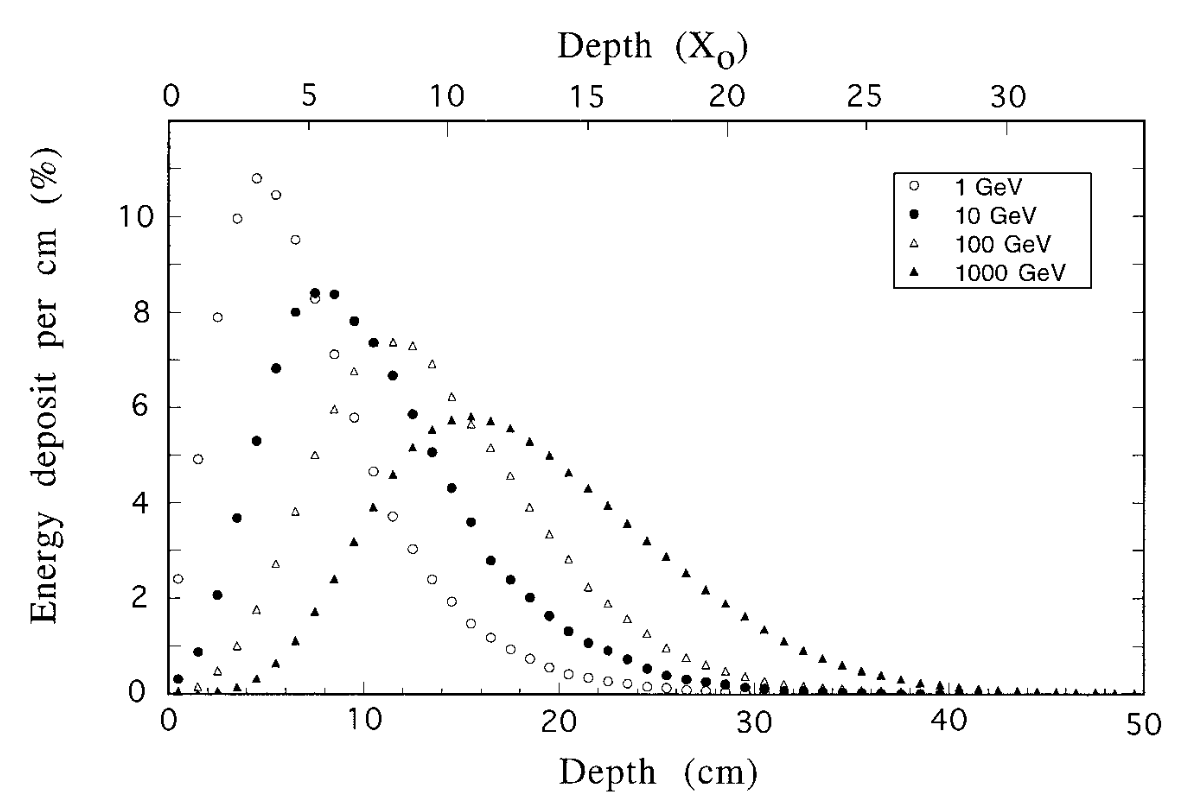
\includegraphics[width=0.7\textwidth]{IMG/Cap2/shower_max.png}
	\caption{The energy deposit as a function of depth, for $1$, $10$, $100$ and $1000\ GeV$ electron showers developing in a block of copper \cite{Leo}.}
	\label{fig:shower_max}
\end{figure}

Another quantity useful to describe the spatial shower development, in particular the transverse one, is the Molière radius. It is defined in terms of the radiation length and the critical energy:
\begin{equation}
    \rho_M = E_s \frac{X_0}{\varepsilon_c}
\end{equation}
where $E_s$ is defined as $m_c^2\sqrt{4\pi/\alpha} \simeq 21.2\ MeV$. This quantity is almost material-independent and, on average, a cylindrical volume with this radius around the shower axis contains $90\%$ of the shower energy. The lateral spread is mainly due to two effects: at high energy, electrons and positrons are moved away from the shower axis because of the deviation occurring in Compton scattering; photons and electrons are also produced in isotropic processes moving them away from the axis (spread more important in lower energy particles). Also brehemstralung process produces photons with a certain angle, contributing to the shower spread. Figure \ref{fig:shower_moliere} give an idea of the radial distribution of deposited energy.\\

\begin{figure}
	\centering
	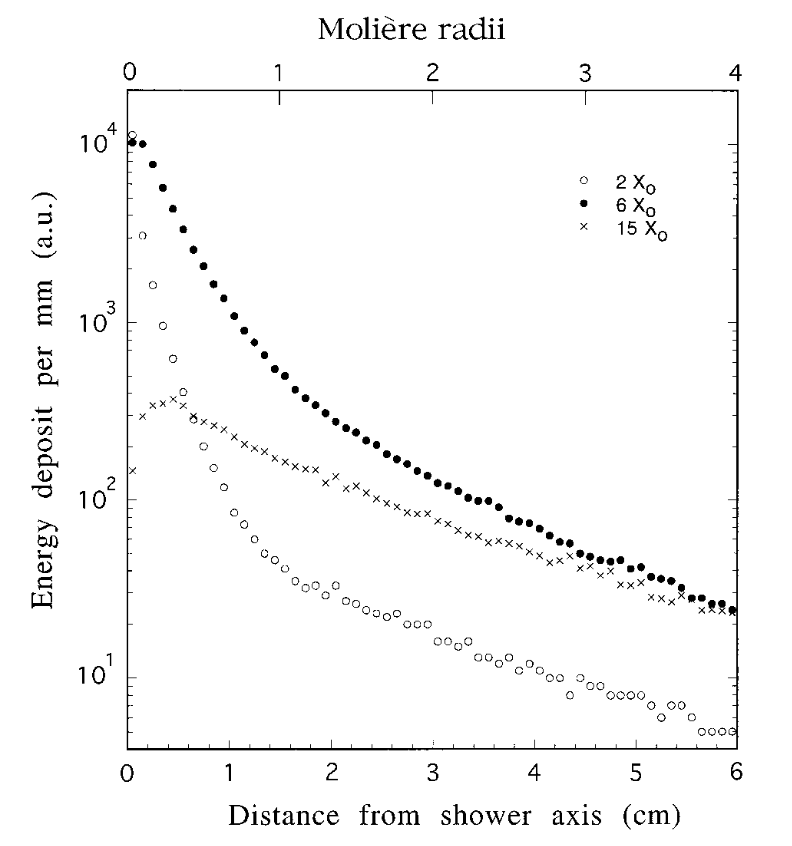
\includegraphics[width=0.6\textwidth]{IMG/Cap2/shower_moliere.png}
	\caption{The radial distributions of the energy deposited by $10\ GeV$ electron showers in copper, at various depths \cite{Leo}.}
	\label{fig:shower_moliere}
\end{figure}

The lateral and longitudinal shower development generated by charged particles and by neutral ones are basically identical except for the initial stages. Electrons start radiating as soon as they enter the calorimeter, instead photons must convert before releasing any energy. Once they start producing electrons and positrons, they can release even more energy than electron induced showers. This behaviour is shown in Figure  \ref{fig:em_start}, where the distribution of the energy fraction deposited in the first $5\ X_0$ by $10\ GeV$ electrons and photons in lead is plotted.

\begin{figure}
	\centering
	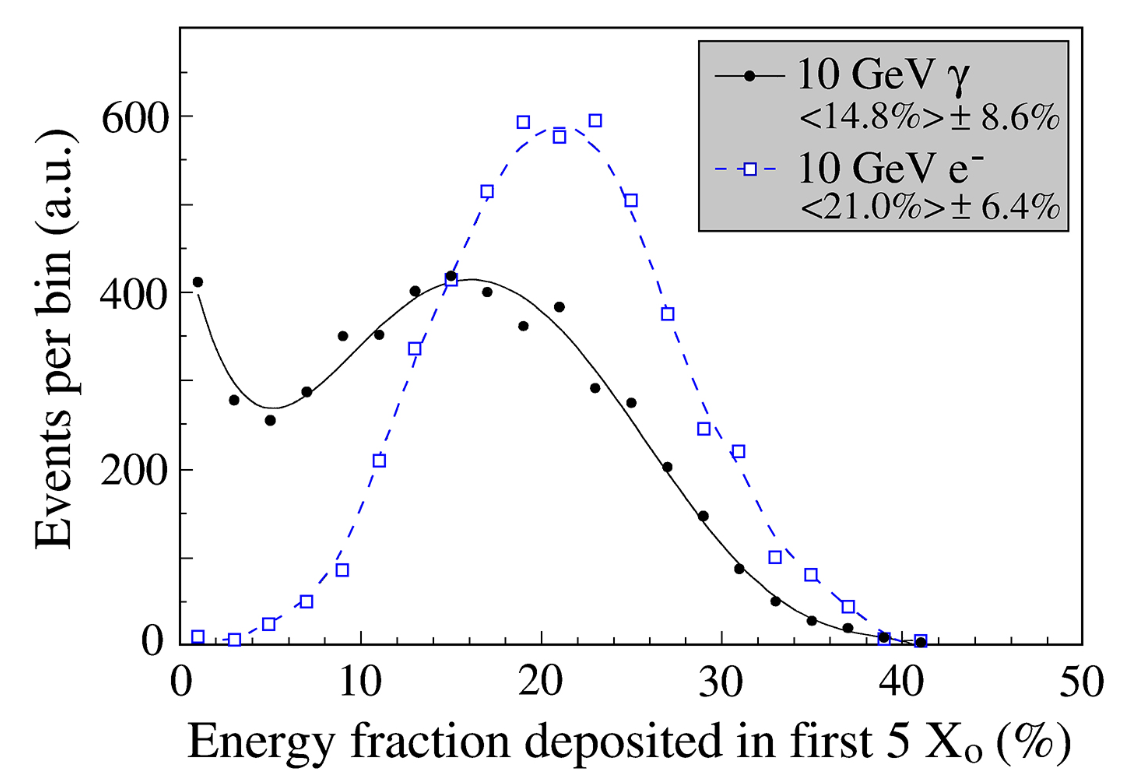
\includegraphics[width=0.7\textwidth]{IMG/Cap2/em_start.png}
	\caption{Distribution of the energy fraction deposited in the first $5\ X_0$ by  $10\ GeV$ electrons and photons showering in lead. Image from \cite{Wigmans_e_gamma}.}
	\label{fig:em_start}
\end{figure}

\subsection{Hadronic showers} \label{subsec:had_shower}
Introducing the hadronic showers a new degree of complexity arises. The showers produced by hadrons are affected by the strong interaction. This interaction is responsible for:
\begin{itemize}
    \item The production of hadronic secondary particles, most of which, $\simeq 90\%$, are pions. Neutral pions mainly decay in two photons, which develop electromagnetic showers.
    \item The occurrence of nuclear reactions where atomic nuclei release neutrons and protons. The fraction of the shower energy needed to unbind the nucleons does not contribute to the energy released to the calorimeter (invisible energy phenomenon).
\end{itemize}
The part of energy released via electromagnetic showers is commonly named em fraction ($f_{em}$), and once the energy is converted to em showers it can not be transformed back to hadronic energy. Another contribution to the complexity is given by the variability of this em fraction event by event and its energy dependence. On average, $f_{em}$ increases with the primary particle energy, since $\pi$s may also be produced by secondary and higher-order particles: the higher the energy, the more the generations of shower particles, the larger the em fraction. The  average  electromagnetic fraction has been evaluated to increase with the energy following the power law:
\begin{equation}
    f_{em} = 1 -1\left(\frac{E}{E_0}\right)^{k-1}
\end{equation}
where $K\simeq 0.82$ and $E_0$ is a matter dependent value of the order of $GeV$. The behaviour in lead and copper is shown in figure \ref{fig:f_em}.\\
In the calorimetry context, these characteristics have important consequences:
\begin{itemize}
    \item \textit{Non-compensation}; the calorimeter signals for hadrons and for electrons of the same energy are in general different a result of the invisible-energy phenomenon, in particular the one for hadrons is generally smaller.
    \item \textit{Non-linearity}; a calorimeter for hadron detection does not present a linear response with respect to the primary particle due to the energy dependence of the em fraction.
\end{itemize}

\begin{figure}
	\centering
	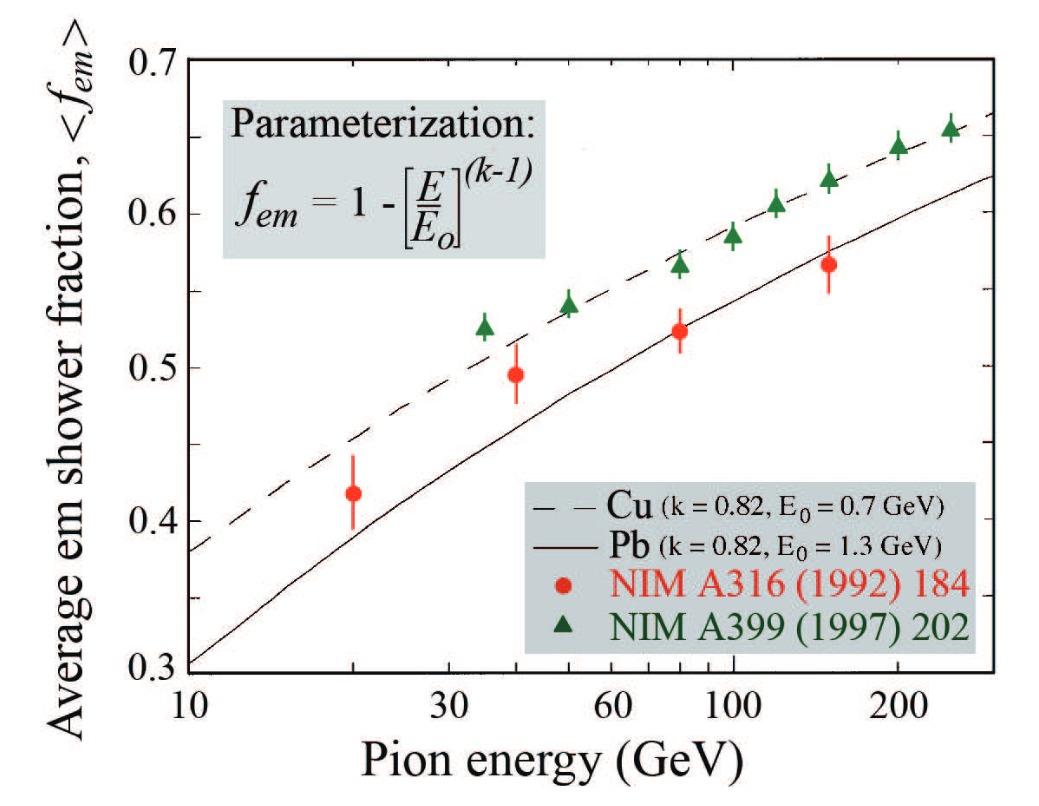
\includegraphics[width=0.7\textwidth]{IMG/Cap2/f_em.png}
	\caption{Comparison between the experimental results on the em fraction of pion-induced showers in copper-based and lead-based calorimeters. Image from \cite{fem_par}.}
	\label{fig:f_em}
\end{figure}

Another important difference between em and hadronic showers is the greater spatial profiles of released energy. Analyzing for example several pions traces, peaks of signals are produced at a depth near the one where a $\pi^0$ is generated. However, the neutral pion production can occur in the second or third generation of the shower development releasing energy at different depth. An example of $4$ different showers from $270\ GeV$ pions is illustrated in figure \ref{fig:had_start}.\\
The depth of the calorimeter required to contain hadronic showers increases logarithmically with energy, as already seen for em showers, but the large longitudinal fluctuations make the leakage effect a point of extreme interest also in configuration that would contain, on average, $99\%$ of the shower.\\
Laterally, an hadronic shower is easier contained if the primary particle has higher energy. This is due to the fact that the electromagnetic shower fraction increases with energy. The em showers produced tend to develop laterally close to the shower axis.
 
 \begin{figure}
	\centering
	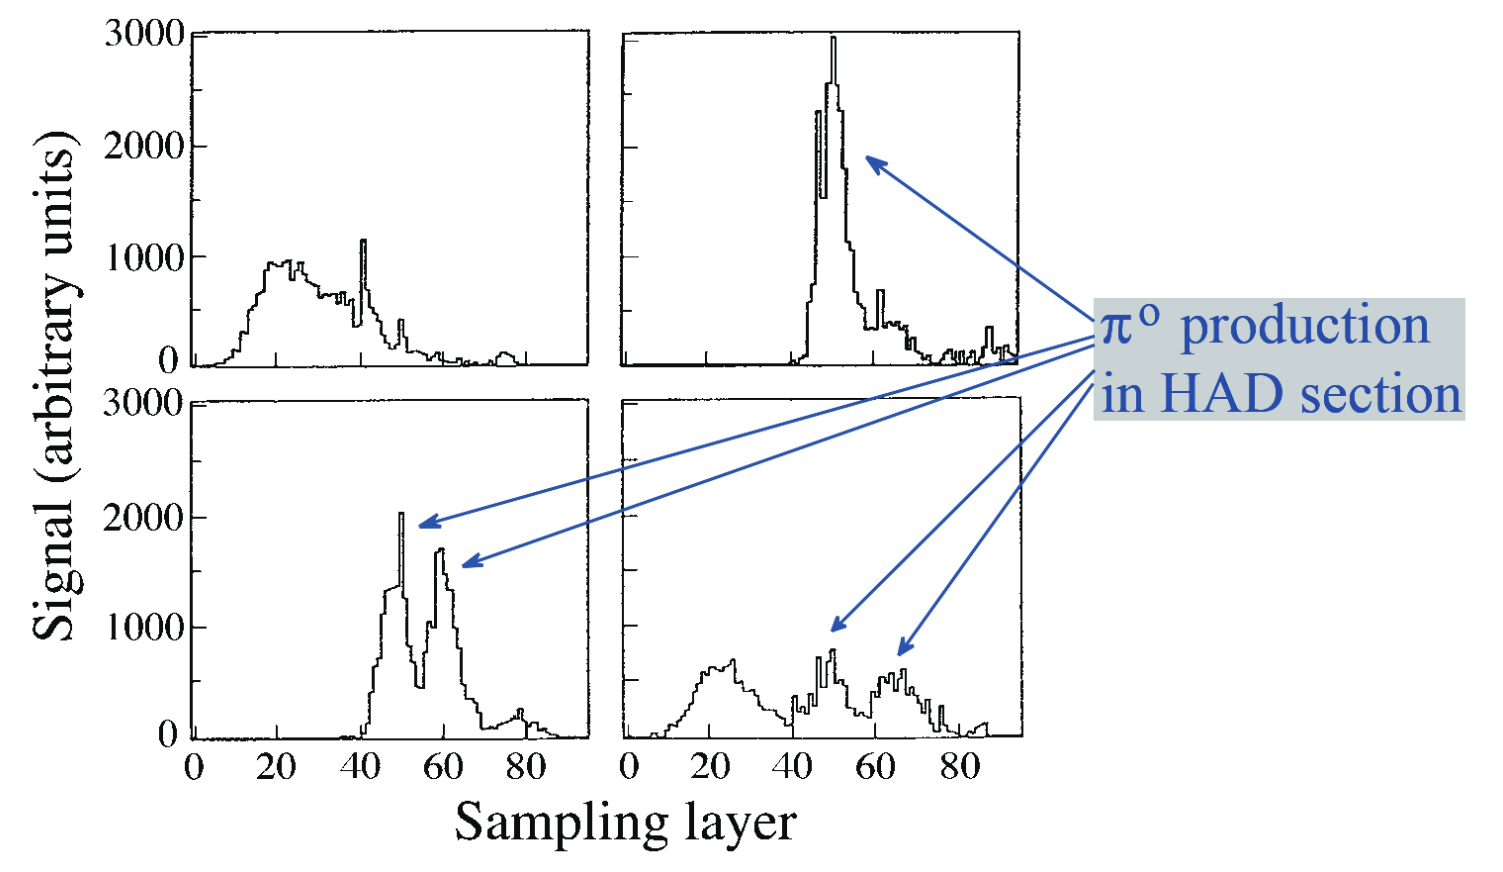
\includegraphics[width=0.7\textwidth]{IMG/Cap2/had_start.png}
	\caption{Longitudinal  profiles  for  $4$  different  showers  induced  by  $270\ GeV$  pions  in  a  lead/iron/plastic-scintillator calorimeter \cite{Wigmans_art_of_cal}.}
	\label{fig:had_start}
\end{figure}

\section{Energy response of calorimeters}
Starting from the definition of the term \textit{response}, it is the average calorimeter signal per unit of deposited energy. The response is usually expressed in  terms, for example, of number of photoelectrons per $GeV$ or charge ($pC$) per  $MeV$. A straight forward definition is the linearity of a calorimeter, it is defined \textit{linear} if its response is constant.\\

\subsection*{Electromagnetic calorimeters}
Electromagnetic calorimeters are detector optimized to induce em showers. In these showers, all the energy carried by the primary particle is released by a very large number of shower particles through processes that may generate signals (excitation or ionization in the absorbing medium). The number of particles is on average proportional to the primary energy and the signal generated by each one of these is established by the detector properties. The direct consequence is that em calorimeters are in general linear detectors.\\
A non-linearity response is usually an indication of instrumental problems. The most common ones are:
\begin{itemize}
    \item leakage effects, caused by too small dimensions of the calorimeter;
    \item saturation effects of the active components, originated by possible high localized energy depositions;
    \item recombination of electrons and ions, making the energy carried by the electron undetected.
\end{itemize}

At the same time, the small lateral and longitudinal em shower development allows to design relatively small calorimeters, often used as electromagnetic components in more complex systems.\\

A structural distinction can be made between \textit{homogeneous} and \textit{sampling} calorimeter.\\
The main advantage of homogeneous detectors is their excellent energy resolution, achievable because the whole energy of the primary particle is released in the active medium. At the same time, if a well position measurement and particle identification are required, homogeneous calorimeters are not the best choice because of the challenging lateral and longitudinal segmentation task. 
Homogeneous calorimeter can be classified in four groups:
\begin{itemize}
    \item semiconductor calorimeters;
    \item Cherenkov calorimeters;
    \item scintillator calorimeters;
    \item noble-liquid calorimeters.
\end{itemize}

On the other hand, sampling calorimeters have in general worst energy resolution due to the presence of an absorber material (copper, iron, lead or uranium) that does not contribute to produce the signal and the sampling fluctuations. For electromagnetic sampling calorimeters, typical resolution values are in the range of $5-20 \% / \sqrt{E(GeV)}$. Meanwhile they are relatively simple to segment longitudinally and laterally due to their sampled structure contributing to achieve a better space resolution. Although this structure can be used to reduce the em calorimeter sizes, they are universally used in hadronic calorimeters.

\subsection*{Hadronic calorimeters}
Hadronic calorimeters are detector optimized to induce hadronic showers, are more complex because both em and hadronic shower are produced in them. The calorimeter response is, therefore, divided in em ($e$) and non-em ($h$) components. The ratio $e/h$ classifies calorimeters in three categories: \textit{compensating}, if $e/h=1$; \textit{undercompensating}, if $e/h>1$; \textit{overcompensating}, if $e/h<1$. Hence, the total calorimeter response (to charged pions) is a combination of the two:
\begin{equation}
    \pi = f_{em} \cdot e + (1- f_{em}) \cdot h.
\end{equation}
Since the average $f_{em}$ value, as already seen, increases with the energy, a non-compensating calorimeter response ($e/h \neq  1$) is not constant and hence non-compensating calorimeters are intrinsically non-linear detectors.
The $e/h$ value cannot be directly measured. However, it can be derived from the $e/\pi$ ratios, measured at various energies. The relationship between $e/\pi$ and $e/h$ is as follows, where $f_{em}$ is the energy dependent average em fraction:
\begin{equation}
    \frac{e}{\pi} = \frac{e/h}{1 - f_{em}(1-e/h)},
\end{equation}
the relation is represented in figure \ref{fig:compensation}.

 \begin{figure}
	\centering
	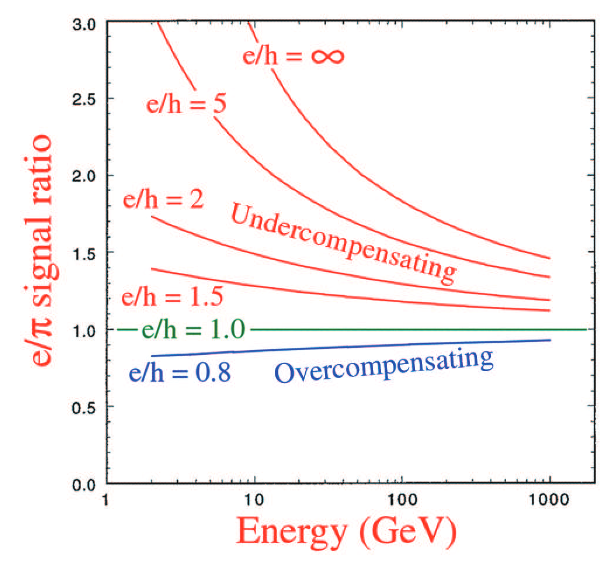
\includegraphics[width=0.65\textwidth]{IMG/Cap2/compensation.png}
	\caption{Relation between the calorimeter response ratio to em and non-em energy deposits, $e/h$, and the measured $e/\pi$ signal ratios \cite{Wigmans_art_of_cal}.}
	\label{fig:compensation}
\end{figure}

The basic reason for different response for em and hadronic showers lies in the fact that in the absorption of hadronic showers, a significant fraction of the energy is \textit{invisible} not contributing to the calorimeter signal. The main source of this energy is the energy used to release nucleons from nuclei.\\
To design a linear calorimeter various compensation methods have been developed. There are two main approach to obtain $e/h = 1$: one is reducing the electromagnetic response and the other one is to increase the non-em response.\\
The most effective way to reduce the em response of a sampling calorimeter is to use an high-$Z$ material as absorber. The concept is based on the way that low energy photons release their energy. As seen, the main process at low energies is the photoelectric effect that is highly $Z$ dependent. For this reason, using high-$Z$ absorber materials causes an energy deposition in the absorber making this energy not detected.\\
The other strategy is known as compensation by neutrons signal boosting or by Signal Amplification through Neutron Detection (SAND). It consist in increasing the non-em response taking advantage of the kinetic energy transported by neutrons. The good correlation between the invisible energy and the kinetic energy of neurons opens the possibility of an event-by-event correction boosting the signals generated by the neurons. The most likely process that occur at low energies for a neutron is elastic scattering on a nucleus target. The fraction of energy transferred in this process is on average $f_{\text{elastic}} = 2A / (A +1)^2$ (where $A$ is the mass number of the target). Considering that hydrogen maximize this fraction it is the element that must be present in the active medium to produce the non-em response increment. With this consideration and fine tuning the sampling fraction, a $e/h$ ratio can be forced to be $1$ obtaining a linear hadronic calorimeter.
In short, compensation through SAND can be achieved in sampling calorimeters with active materials containing hydrogen and a precisely tuned sampling fraction.\\
In the IDEA dual-readout calorimeter, a more recent compensation strategy is designed. The dual-readout compensation used will be described in section \ref{sec:DRComp}.

\subsection{Fluctuations}
The energy response of a calorimeter represent an average value, but the energy loss is a statistical phenomenon therefore the precision of these detectors is affected and limited by fluctuations. The effect is quantified by the relative resolution defined as the energy distribution standard deviation divided by the mean value ($\sigma/E$).\\
Considering the simpler case of em calorimeters, four are the main sources of fluctuation:
\begin{itemize}
    \item sampling fluctuations;
    \item signal quantum fluctuations;
    \item shower leakage fluctuations;
    \item instrumental fluctuations.
\end{itemize}
Sampling effects are affected both by the sampling fraction (i.e. the ratio of the active material on the total) and the sampling frequency (the thickness of the layers). The sampling fraction is  defined as:
\begin{equation}
    f_{samp} = \frac{E_{active}}{E_{passive}+E_{active}}
\end{equation}
where $E_{active}$ and $E_{passive}$ are the energies deposited in the active and passive part by an incident minimum ionizing particle (mip).
This type of fluctuation is dominated by the Poisson statistics, hence it contribute with a term proportional to $1/\sqrt{E}$ to the energy resolution.
In em calorimeter with non-gaseous active material the sampling contribution follow the empirical law:
\begin{equation}
    \frac{\sigma}{E} = \frac{2.7\% \sqrt{d/f_{samp}}}{\sqrt{E}}
\end{equation}
where $d$ is the thickness of the active material layer measured in $mm$.\\
Fluctuation effects due, for example, to photon statistics in light emitting active materials are grouped under the label of signal quantum fluctuations. Also these fluctuations follow the rules of Poisson statistics, with the constrain of uncorrelated separate contributions. Another contribution that scales with $E^{-1/2}$ is added to the relative energy resolution expression.\\
In leakage fluctuations there are three possibilities: longitudinal, lateral and albedo. These fluctuation are highly dependent to the geometry and the material of the calorimeter. For this reason their contribution to the resolution does not have a precise energy dependent form. The typical solution to numerically evaluate their effect is to produce Monte Carlo simulation for the calorimeter and study the obtained data.\\
Finally, instrumental fluctuations are the ones provided, for example, by electronic noise or geometrical inhomogeneities. The electronic noise contribution is usually described with a term that scales with $1/E$ because it is largely independent of the shower energy. Meanwhile fluctuations induced by structural inhomogeneities depend on the shower position and might be energy dependent.\\
Typically, these contribution are uncorrelated and have to be added in quadrature to obtain the total resolution. As seen, different contribution with different energy dependence have to be considered. The consequence is that different effects dominate the energy resolution in different energy ranges. These behaviour have to be considered in the design of the calorimeter in order to optimize the resources.\\

All the sources described affect also hadronic calorimeters. For example, sampling fluctuation has a higher impact in hadronic showers due mainly to the lower average number of particle that release energy in the hadronic ones. 
At the same time, in hadronic detectors, resolution is affected also by other fluctuation effects.\\
The introduction of quantities such as $f_{em}$ in hadronic calorimeters produces new sources of fluctuations. In non-compensating calorimeter, event-by-event fluctuation in em component affect the detector response. It contributes to the relative energy resolution through a term scaling as $c E^{-0.28}$.
\begin{equation}
    \frac{\sigma}{E} = \frac{a_1}{\sqrt{E}} \oplus c E^{-0.28}
\end{equation}
Up to $400 GeV$, this law runs almost parallel to an energy resolution in which only the stochastic term is included ($\sigma/E = a/\sqrt{E}$). For this reason, the resolution of non-compensating calorimeter is often described as:
\begin{equation}
    \frac{\sigma}{E} = \frac{a_2}{\sqrt{E}} + b.
\end{equation}
A useful solution that remove these fluctuations is to design a compensating calorimeter, greatly improving the energy resolution.\\
Finally, the calorimeter resolution is also affected by invisible energy fluctuations. To evaluate the impact of these fluctuations the correlation between $f_{em}$ and $f_{inv}$ has to be known, and in particular if they are correlated or not. If they are uncorrelated the contribution to the resolution has to be added in quadrature. Moreover, in compensating calorimeter, the contribution of invisible energy fluctuations are different depending on the techniques used to achieve compensation.

\section{Dual-readout compensation}\label{sec:DRComp}
All the benefits obtained with compensating calorimeters are obtaining by sampling em and non-em components in hadronic showers with the same response ($e=h$). Dual-readout is a method that perform this correction event-by-event, constantly measuring the electromagnetic fraction \cite{DR_Wig}. 

\subsection{Working principles}
This technique is based on the concept that the em component is mostly provided by relativistic electrons and positrons, while the majority of non-em one is carried by non-relativistic particles. Hence, collecting the Cherenkov signal produced by an hadronic shower is almost equivalent to sampling the em component, estimating the electromagnetic fraction. A second simultaneous signal, typically from scintillators, is recorded. Thanks to this second signal, the non-em component can be evaluated starting from the $f_{em}$ already obtained.\\

Entering the details of the process, let's consider scintillation (S) and Cherenkov (C) signals produced by an hadronic shower. The mean values of these signals are calibrated with an electron beam of known energy $E$ so that, for em showers, $\expval{S} = \expval{C} = E$. The hadronic signals can be written (for each event) as:
\begin{align}
    S &= E \left[f_{em} + (h/e)_S (1-f_{em}) \right], \label{eq:S} \\
    C &= E \left[f_{em} + (h/e)_C (1-f_{em}) \right], \label{eq:C}
\end{align}
where $h/e$ quantify the two different degree of non-compensation for the two signals. Considering that $h/e$ are measurable quantities and are assumed to be constants, the ratio $C/S$ is also energy independent:
\begin{equation}
    \frac{S}{C} = \frac{f_{em} + (h/e)_S (1-f_{em})}{f_{em} + (h/e)_C. (1-f_{em})} \label{eq:em_frac}
\end{equation}
This expression can straightforwardly give an evaluation of the em fraction:
\begin{equation}
    f_{em} = \frac{(h/e)_C-(C/S)(h/e)_S}{(C/S)\left[1-(h/e)_S\right]-\left[1-(h/e)_C\right]}
\end{equation}
allowing the rewriting of \ref{eq:S} and \ref{eq:C} as
\begin{align}
    S/E &= (h/e)_S + f_{em}\left[1-(h/e)_S\right], \label{eq:S2} \\
    C/E &= (h/e)_C + f_{em}\left[1-(h/e)_C\right]. \label{eq:C2}
\end{align}

A $C/E$ vs $S/E$ scatter plot can be sketched using signals from a generic DR calorimeter for electrons, pions and protons showers. An example is shown in figure \ref{fig:theta_DR}. As expected, data generated from electrons are always around the point $[1,1]$ (where $f_{em} = 1$). On the other hand an hypothetical signals with only non-em component would be at $[(h/e)_S,(h/e)_C]$ where $f_{em}$ is $0$. Signals from pions and protons showers are clustered along a straight line linking these two points. From this geometric construction it is clear that the slope of this line (the $\theta$ angle) is energy independent because it is determined only by the two $e/h$ values. Thanks to the fact that $\theta$ is energy and particle independent, it is possible to define the parameter:
\begin{equation}
    \chi = \frac{1-(h/e)_S}{1-(h/e)_C} = \cot{\theta},
\end{equation}
this parameter can also easily estimated with test beam data depending only on calorimeter material and geometry.
Finally, event-by-event, the energy of each hadron shower can reconstructed  using the $S$ and $C$ signals in an unique way:
\begin{equation}
    E = \frac{S - \chi C}{1 - \chi}.
\end{equation}

\begin{figure}
	\centering
	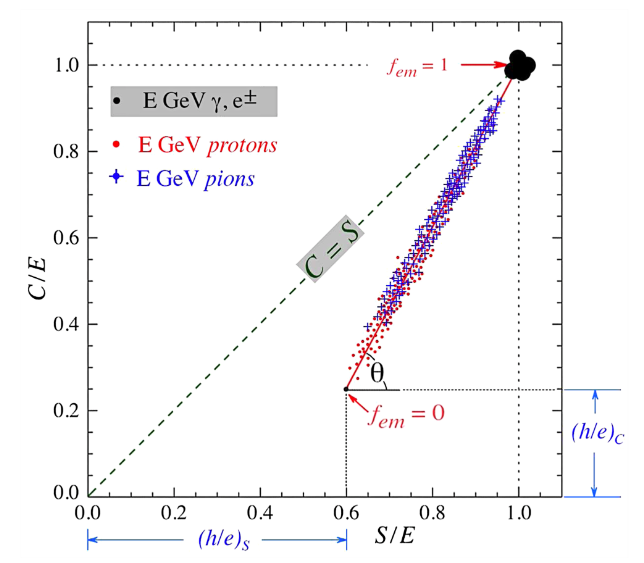
\includegraphics[width=0.65\textwidth]{IMG/Cap2/theta_DR.png}
	\caption{Relation between the calorimeter response ratio to em and non-em energy deposits, $e/h$, and the measured $e/\pi$ signal ratios \cite{DR_Theta}.}
	\label{fig:theta_DR}
\end{figure}

The ideal DR calorimeter is able to identify the Cherenkov signal as the exact electromagnetic component ($h/e = 0$) being a direct measurement of $f_{em}$. The worst DR calorimeter instead is designed when $(h/e)_C = (h/e)_S$, in this case the two signals would sample the two components (em and non-em) with the same response giving no information about the $f_{em}$ from the $S/C$ ratio.  Therefore, the best real DR calorimeter is the one with the lower $\chi$ parameter found with the lower $(h/e)_C$ and the higher $(h/e)_S$ values possible. 

\subsection{Experiments}
At present a few dual-readout calorimeter have been built and tested, and more project are under study.\\
The first practical usefulness of the dual-readout method was tested in a R\&D study for the Advanced Cosmic Composition Experiment at the Space Station (ACCESS) \cite{ACCESS}. The prototype had a depth of $1.4\lambda_{int}$ and was equipped with both plastic-scintillator ($S$) and quartz ($Q$) optical fibres to measure and collect the scintillation and Cherenkov light, respectively. With this detector, the $Q/S$ signals ratio was found to represent a good event-by-event measurement of the shower energy fraction carried by $\pi^0$.\\
Later, a $10 \lambda_{int}$ deep calorimeter known as Dual-REAdout Method (DREAM) was built and tested \cite{DREAM1, DREAM2}. 
The detector is composed by $5580$ basic element represented in figure \ref{fig:DREAM}. These are $200\ cm$ long, hollow, extruded copper rod of $4\times 4 mm^2$ cross section in which $3$ scintillating and $4$ Cherenkov fibres are inserted.
\begin{figure}
	\centering
	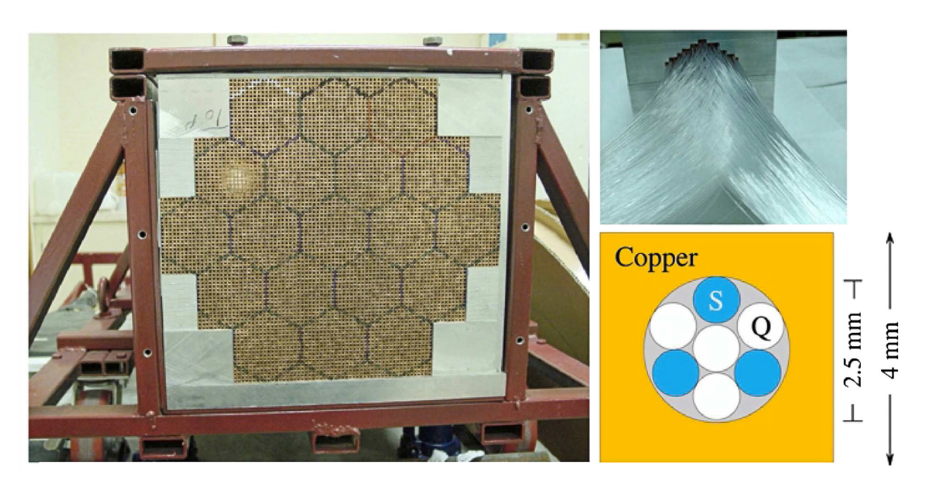
\includegraphics[width=0.65\textwidth]{IMG/Cap2/DREAM.png}
	\caption{The DREAM calorimeter layout \cite{DREAM}.}
	\label{fig:DREAM}
\end{figure}

Figure \ref{fig:theta_DREAM} shows the $C-S$ scatter plot of the calibrated signals, where the correlation between them its clear.
The two $h/e$ ratios for Cherenkov and scintillator DREAM structures are $0.21$ and $0.77$, respectively. The expression of the em fraction \ref{eq:em_frac} becomes:
%\begin{equation}
%    \frac{C}{S} = \frac{f_{em} + 0.12 (1-f_{em})}{f_{em} + 0.77 (1-f_{em})}.
%\end{equation}
\begin{equation}
    f_{em} = \frac{0.21-0.77(C/S)}{(C/S)\left[1-0.77\right]-\left[1-0.21\right]}
\end{equation}

\begin{figure}
	\centering
	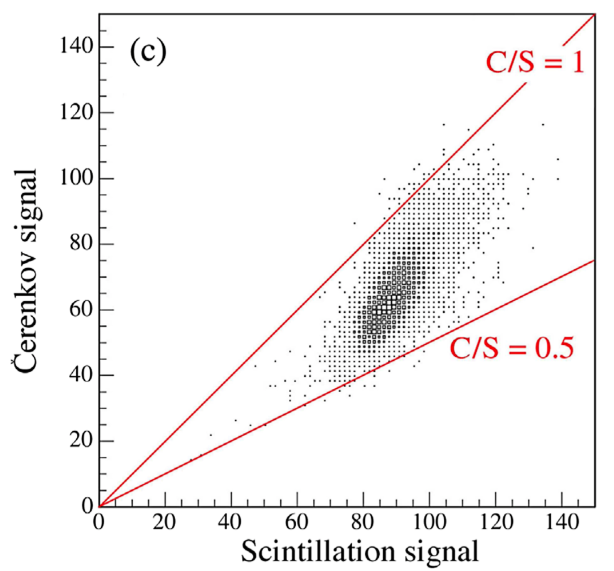
\includegraphics[width=0.65\textwidth]{IMG/Cap2/theta_DREAM.png}
	\caption{ The $C-S$ scatter plot showing the correlation between both types of signals. The signals are expressed in the same units used to calibrate the calorimeter (em GeV) \cite{DREAM2}.}
	\label{fig:theta_DREAM}
\end{figure}

The DREAM results, together with other studies (e.g. SPACAL and RD52) confirmed the potentiality and the good concept of the dual-readout compensation method, bringing to the IDEA dual-readout calorimetry project.